\documentclass[11pt]{article}

% First load extension packages
\usepackage[a4paper,margin=25mm]{geometry}    % page layout
\usepackage{setspace} \onehalfspacing         % line spacing
\usepackage{amsfonts,amssymb,amsmath}         % useful math extensions
\usepackage{graphicx}                         % graphics import
\usepackage{siunitx}                          % easy SI units
\usepackage{url}
\usepackage{wrapfig}
\usepackage{float}

% Change paragraph indentation
\setlength{\parskip}{10pt}
\setlength{\parindent}{0pt}

% User-defined commands
\newcommand{\diff}[2]{\frac{\mathrm{d}{#1}}{\mathrm{d}{#2}}}
\newcommand{\ddiff}[2]{\frac{\mathrm{d}^2{#1}}{\mathrm{d}{#2}^2}}
\newcommand{\pdiff}[2]{\frac{\partial{#1}}{\partial{#2}}}
\newcommand{\pddiff}[2]{\frac{\partial^2{#1}}{\partial{#2}^2}}
\newcommand{\pdiffdiff}[3]{\frac{\partial^2{#1}}{\partial{#2}\partial{#3}}}
\renewcommand{\vec}[1]{\boldsymbol{#1}}
\newcommand{\Idx}{\;\mathrm{d}x}
\newcommand{\Real}{\mathbb{R}}
\newcommand{\Complex}{\mathbb{C}}
\newcommand{\Rational}{\mathbb{Q}}
\newcommand{\Integer}{\mathbb{Z}}
\newcommand{\Natural}{\mathbb{N}}

% topmatter
\title{3D Object Detection in the Wild}

\author{Matt Clifford \\ Supervised by Dr R.\ Santos-Rodriguez}

\date{\today}

% main body
\begin{document}
\maketitle

\section{Introduction}
Explain why 3D object detection is important... cars... 2D is a simplification of the world, 3D gives us a better understanding.



With recent advancements in mixed reality technology from Google glass and Microsoft HoloLens, there is an interest in the use of mixed reality to help create `smart spaces', where mixed reality users are informed and guided through environments unknown to them, addressing circulation issues, or aiding the visually or navigationally impaired.

Fracture Reality \cite{fracture}, has specific interest in 3D object detection for future projects. They specialise in creating bespoke mixed reality software for both private and government sectors. They mostly work with mixed reality visualisations of maps of an environment, for example to aid the control centres in airports \cite{youtube}. Although they have many projects that would benefit from 3D object detection, an ongoing project investigating how effective the use of mixed reality is in tackling navigational issues of fire fighters in buildings unknown to them. The use of 3D object detection would identify and locate objects such as stairs, doors and elevators. This would aid the fire fighter in identifying if these objects are correct pathway for them, without them having detailed prior knowledge of the building, since a map can be stored on the mixed reality device.

Fracture Reality are able to create some object specific use case data, but in the region of hundreds of examples, and due to the specificity of each task, finding existing object datasets might not be possible. This leaves retraining a detector for every new object is infeasible. The need for a system that can detect objects given as little training examples as possible is therefore needed. This can be achieved by utilising general knowledge learnt from similar or relevant tasks and quickly applying it to the specific task of interest \cite{DeCAF}.

Since objects of interest for the object detection are on a case to case basis, due to specific needs of each project. All that is certain, is that the objects are going to be in a real life setting. Therefore there is a need for a robust 3D object detection system that can cope in the wild, where object labels might not be clear and can change over time.



\section{Literature review}
\subsection*{2D Image Classification}
In 2012, Alex Krizhevsky et al. revolutionised computer vision with a convolution neural network (CNN), inspired by \cite{Yann}. It performed image classification on the ImageNet dataset \cite{ILSVRC15}. The CNN, named AlexNet, consists of 5 convolution layers followed by 3 fully-connected layers. It won ImageNet's ILSVRC-2010 and ILSVRC-2012 image classification contests \cite{alex_net}. In \cite{alex_net}, they claim `All of our experiments suggest that our results can be improved simply by waiting for faster GPUs and bigger datasets to become available', and since AlexNet's success there have been consistent advancements in CNN state of the art. In 2014, \cite{VGG16} propose a CNN named VGG16, consisting of 16 convolution layers followed by 3 fully-connected layers. VGG16 achieves a top-5 error rate of 7.4\% on ILSVRC-2014 compared to AlexNet's 17.0\%. \cite{VGG16} achieves this performance boost by using smaller convolution filters, 3x3 compared to AlexNet's 11x11 which decreases the number of weights to train at each convolution layer, alongside a deeper convolution architecture, which can extract deeper relevant semantic meaning from the images. Further performance improvements were made by the use of `inception models' \cite{inception}\cite{inceptionV2}, which stack the outputs of several convolutions of the same input, followed by filter concatenation. As well as `residual learning' \cite{ResNet}, which connects the outputs of multiple convolution layer. \cite{Incep_ResNet} formulates a combination of `inception' and `residual' models. Further improvements to 2D image classification include \cite{neural_search} \cite{scaleable_image}.

\subsection*{2D Object Detection}
To identify the location of objects in images, \cite{RNN} uses a regional CNN (RCNN) model. Regional proposals of the image, which are run though a modified AlexNet. The positive classification results from the regional proposals are then adjusted using a linear regression model to obtain better object bounding boxes. Computational speed ups are proposed in Fast-RNN \cite{fast_RNN}, which pools the regional proposals. Further computational speed ups are proposed in Faster-RNN \cite{faster_RNN}, which combines the selective search regional proposals into the CNN. \cite{YOLO} proposes a grid search grid method rather than the more expensive regional proposals approach, known as `you only look once' (YOLO).

\subsection*{3D Object Detection}
\cite{complex_YOLO} proposes a method of using the YOLO object detection approach in 3D space named Complex-YOLO, using only point cloud data from LIDAR depth sensors. Complex-YOLO uses a Euler-Region Proposal Network which estimates the orientation of objects by adding an imaginary and real part for each proposal box box. This results in 5 times speed up in object detection from the previous state of the art, with on par or better accuracy evaluated on data from KITTI benchmark suit \cite{KITTI}. Other state of the art methods based the KITTI benchmark suite include \cite{point_fusion}\cite{multi_fusion}\cite{fast_furious}\cite{VoxelNet}. 

Some methods focus on using detailed, accurate point cloud objects as input \cite{subgroup_voting}\cite{pose_RGBD}\cite{real_time_single} from datasets such as \cite{3D_dataset}. Using this type of model directly is unsuitable for mixed reality, as there is little background variation which makes them not robust enough for detection in the wild. 

\cite{PointNets} and \cite{frustum} use 2D object detectors to aid the regional proposal of the 3D object, by searching only the 3D space in the point cloud occupied from the projected frustum obtained from the 2D object detector. This vastly reduces the search space. Resulting in reduced misclassification, due to the higher accuracy of 2D detection, especially if the 3D object suffers from occlusions or has a sparse representation. Speed is also improved when compared to using point cloud data alone, due to the pre determination of the object class and reduced search space for the 3D detector. An alternative approach could combine 2D object mask detectors\cite{first_person_mask}\cite{mask_RCNN} with the 3D projection of the mask to help further refine the 3D object search space. \cite{latent_surface} uses latent support surfaces for 3D object detection on the SUNRGBD dataset. Another notable 3D object detector that use the SUNRGBD dataset is \cite{SnapNet}. 

\subsection*{Transfer Learning}
Transfer learning is a well studied area of deep learning \cite{DeCAF}\cite{survery_on_transfer}\cite{how_transferable}, where a network trained for a specific task is re-purposed for a similar task. This is often achieved by truncating the last few layers of a pre-trained network where the network is specific to the trained task, and keeping the starting layers that have more general representations. Since the start of the network is already trained for general tasks relevant to both the original training task and the new desired task, only the last few layers need to be re-trained for the new task. This can be done using considerably less training data than the original network was trained with. Transfer learning could be used to help solve the problem of using as little 3D data as possible to train a 3D object detector. However, when using as little data as possible during the retraining part of transfer learning, the original network needs to be trained for a task as similar as possible as the re-purposed task.

\subsection*{Synthetic Data}
\cite{cut_paste} proposes a `cut and paste' style approach to synthesising 2D object detection datasets. First an object mask is predicted for the object, which is then applied to the image to `cut and paste' the object into background scenes. Occlusions, truncations and blends are then applied to the object, helping it fit more naturally into the scene. This address' the problem of not being able to annotate or collect enough data by hand. \cite{synthetic_train} shows that training scene detectors on synthetic data produces comparable results on real life tests, with object detectors trained on the SUNRGBD state of the art dataset.

Common representation -- do a little research,,
	Auto encoders to possibly solve this 

Unsupervised learning for creating data cheaply


\section{Project plan}

- collect dataset

- CNN as baseline for classification

- faster-RCNN as baseline for 2D object detection

- Make baseline 3D object detector using point cloud data

- Transfer 2D model to 3D, elaborate on this

- Assess results of transfer learning 3D detector with a few 3D new object examples

- Auto-encoder to find common representation between 2D and 3D?

- Generating objects in scenes using cut and paste in 3D?

\section{Progress}
\subsection*{Datasets}
The KITTI benchmark suit \cite{KITTI} is an autonomous driving dataset with 200,000 3D object annotations captured in cluttered scenarios, with up to 15 cars and 30 pedestrians in each image. The data is obtained from a stereo camera and LIDAR sensor mounted on top of a car that is driven in the real world. Although the KITTI benchmark suit is a rich 3D object dataset, it is not as directly applicable to mixed reality application due to the sensing quality differences between LIDAR and the portable depth camera used in mixed reality. As well as KITTI only focusing on 8 autonomous driving classes such as pedestrians, cars and bicycles. 

\cite{3D_dataset} is a large-scale 3D object dataset with 32040 object poses and 45 different objects. The point cloud data is triangulated from 11 different views, making highly detailed scenes. The scenes are controlled and do not represent what would be captured from mixed reality depth sensors due to the triangulated different views.

SUNRGBD benchmark suite \cite{SUNRGBD} is a 3D object dataset consisting of 10,335 images with 64,595 3D object bounding boxes. The data is collected on various portable RGBD cameras such as the Kinect device, with indoor scenes focusing on objects such as doors, tables and chairs. A similar quality popular dataset is the Pascal Visual Object Classes (VOC)2012 \cite{pascal-voc-2012}, which consists of 11,530 annotated object images, indoors and outdoors with 20 classes such as chairs, cars, dogs. However, PASCAL VOC 2012 only consists of 2D data. \cite{PASCAL_3D} extends the PASCAL VOC 2012 dataset with proposed 3D CAD style projections of the 2D objects. Although rich, this 3D data of the object is dissimilar to that of a depth sensor, leaving SUNRGBD the most suitable starting dataset for this project.

To easily access relevant parts of the dataset a pipeline is made; RGD image, depth image, point cloud, 2D labels and bounding box and 3D labels and bounding box. This data pipeline also includes cropping images to the objects within them, for training an image classifier. Other features include taking a subset of object labels and a subset of these images. This is important, as it simplifies the problem when testing which methods are feasible, before training on the whole dataset.

** show some photos of the sundata set

- show some examples of the dataset with annotations

- show examples of cropped inputs

Show where the is some bad data -  this will be a weakness. Could look into removing these from the dataset, by seeing where any classifier or object detector is failing, as it will most likely be on inaccurately labelled objects.

\subsection*{Image Classification of SUNRGBD objects}
An image classifier is trained on a subset of object classes. As the easiest task, image classification gives an indication of the quality of the dataset and it's annotations, as well as giving an upper bound on what accuracy any object detectors can achieve.

The state of the art InceptionV3 [REF] CNN architecture is used to demonstrate image classification on a subset of the SUNRGB dataset. 500 examples from the classes: chair, door and table are used. In the SUNRGBD dataset, images contain multiple of the same class objects, for example a room full of the same chair. To give a more general representation of objects and the whole dataset, only one object from each image is sampled in a random order of the images. To reduce training time and improve accuracy, weights pre-trained on ImageNet are used. Since ImageNet has 1000 classes, the feature extraction from the network is very general and should apply well to this similar classification task. Transfer learning of the pre-trained InceptionV3 is achieved by truncating the final classification layer and replacing it with the new desired classes. Re-training the weights is achieved by back propagation of the whole network, with batch normalisation and using the cross-entropy loss function. Figure \ref{fig:incept_trans} shows the accuracy of training and validation sets during transfer learning. The model achieves around 94\% accuracy on the validation set. This is very high, and is as expected since the task is very similar to the ImageNet classification task the model was pre-trained on.

\begin{figure}[H]
  \begin{center}
    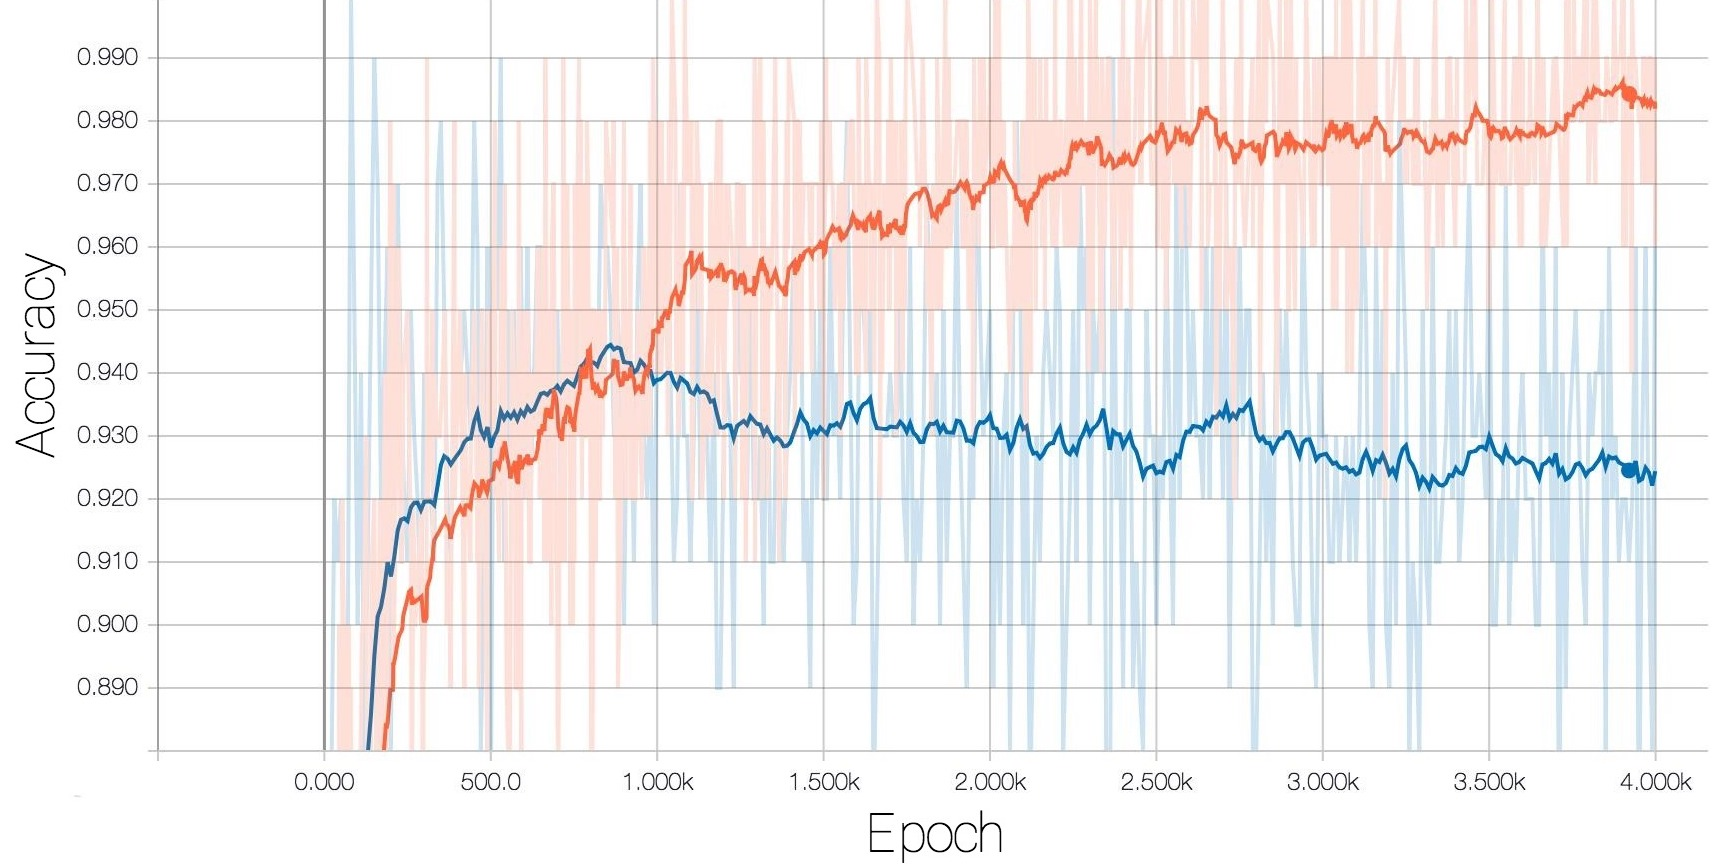
\includegraphics[width=0.9\textwidth]{images/inception_SUNRGBD.jpg}
  \end{center}
  \caption{Accuracy for train set (orange) and validation set (blue) for transfer learning of InceptionV3 with weights pre trained on ImageNet. Both curves are smoothed, with the lighter background colour representing the actual data. The model starts to over-fit after around 800 epochs, where the validation accuracy is seen to decrease from it's peak just above 94\% accuracy.}
  \label{fig:incept_trans}
\end{figure}

%Create the style, and include the bibliography.
\bibliography{interim}
\bibliographystyle{abbrv}

% the end
\end{document}